\documentclass[11pt,a4paper]{article}
\usepackage[utf8]{inputenc}
\usepackage[english]{babel}
\usepackage{amsmath}
\usepackage{amsfonts}
\usepackage{amssymb}
\usepackage{natbib}
\usepackage{graphicx}
\usepackage{cleveref}
\usepackage{enumitem}
\usepackage{listings}
%\usepackage[minionint,frenchmath,mathlf]{MinionPro}
%\usepackage[toc, eqno, enum]{tabfigures}
%\figureversion{lf,tab}
\renewcommand{\familydefault}{\sfdefault}
\usepackage{helvet}
\usepackage{sfmath}
\usepackage[font={small,it}]{caption}
\parindent 0pt
\parskip 12pt
\setcounter{tocdepth}{2}
\setcounter{section}{-1}
\lstset{basicstyle=\ttfamily\small, columns=flexible, breaklines=true}

\begin{document}

\author{Bernhard Bauer-Marschallinger}
\title{\textbf{The Equi7 Grid -- V12 -- Public Package} \\ \vspace{10 mm} \Large \textbf{\textit{Grid Definition Document -- Issue 0.1}}}
\maketitle

%\begin{figure}[hbtp]
%\centering
%\includegraphics[width=1.0\textwidth]{frontpagefigur}
%\end{figure}

\newpage

\parskip 4pt
\tableofcontents

\newpage

\section*{Document History}

\begin{tabular}{llll}
\hline 
\textbf{Issue} & \textbf{Date} & \textbf{Author} & \textbf{Changes} \\ 
\hline 
0.1 & 2014-12-01 & Bernhard Bauer-M. & adopted for Equi7 V12 \\ 
\hline 
\end{tabular} 

\newpage

\section{Preamble}
\label{sec:preamble}

\subsubsection*{Content of Document}
This document describes the design, realisation and software of the Equi7 Grid. This grid was developed at the Department of Geodesy and Geoinformation at the TU~Wien is aimed to use for high resolution remote sensing data. 

\subsubsection*{Scientific Basis}
Detailed information on the scientific background is published under: \\
\textit{B. Bauer-Marschallinger, D. Sabel, W. Wagner: \textbf{Optimisation of global grids for high-resolution remote sensing data.} Computers \& Geosciences, 72 (2014), 84 - 93, DOI: 10.1016/j.cageo.2014.07.005}

\begin{lstlisting}
http://www.sciencedirect.com/science/article/pii/S0098300414001629
\end{lstlisting}

\subsubsection*{Acknowledgements}
This work is the result from efforts spent during ongoing developments carried out at TU Wien across a number of projects and by various staff members. Thanks to FFG, time was found to craft this design document. The major work on the scientific background was carried out in the \textit{Soil Moisture Data Cubes} project. Rendering the grid operational was done in the \textit{Prepare4EODC-Water} project.

\textit{This work has received funding from the Austrian research funding association (FFG) under the scope of the ASAP 9 program within the research project \#840114, Soil Moisture Data Cubes and under the scope of the ASAP 10 program within the research project \#344350, Prepare4EODC-Water.}

\subsubsection*{License}
The Equi7 Grid V12, its software, source files and documentation are licensed under the Creative Commons Attribution-NoDerivatives 4.0 International License. To view a copy of this license, visit

\begin{lstlisting}
http://creativecommons.org/licenses/by-nd/4.0/
\end{lstlisting}

\begin{figure}[hbtp]
\centering

\includegraphics[width=0.2\textwidth]{cc_by-nd}
\end{figure}

\newpage

\parskip 10pt

\section{Overview}
\label{sec:overview}

\subsection{Rationale}
Upcoming remote sensing systems onboard satellites will generate unprecedented volumes of spatial data, hence challenging processing facilities in terms of storage and processing capacities. Thus, an efficient handling of remote sensing data is of vital importance, demanding a well-suited definition of spatial grids for the data's storage and manipulation. For high-resolution image data, regular grids defined by map projections have been identified as practicable, cognisant of their drawbacks due to geometric distortions. 

Further information on the scientific aspect of grid definitions and their suitability to high resolution remote sensing can be found in \cite{Bauer-Marschallinger2014}.

\subsection{Key Facts}
The Equi7 Grid is a spatial reference system for the entire Earth and consists of seven planar subgrids for each continent (Figure \ref{fig:7cont}). The coordinates are defined by individual realisations of the Equidistant Azimuthal projection and are referenced to the ellipsoidal WGS84 datum. The Equi7 Grid is designed to handle efficiently the archiving, processing and display of high resolution remote sensing data.

\begin{figure}[hbtp]
\centering
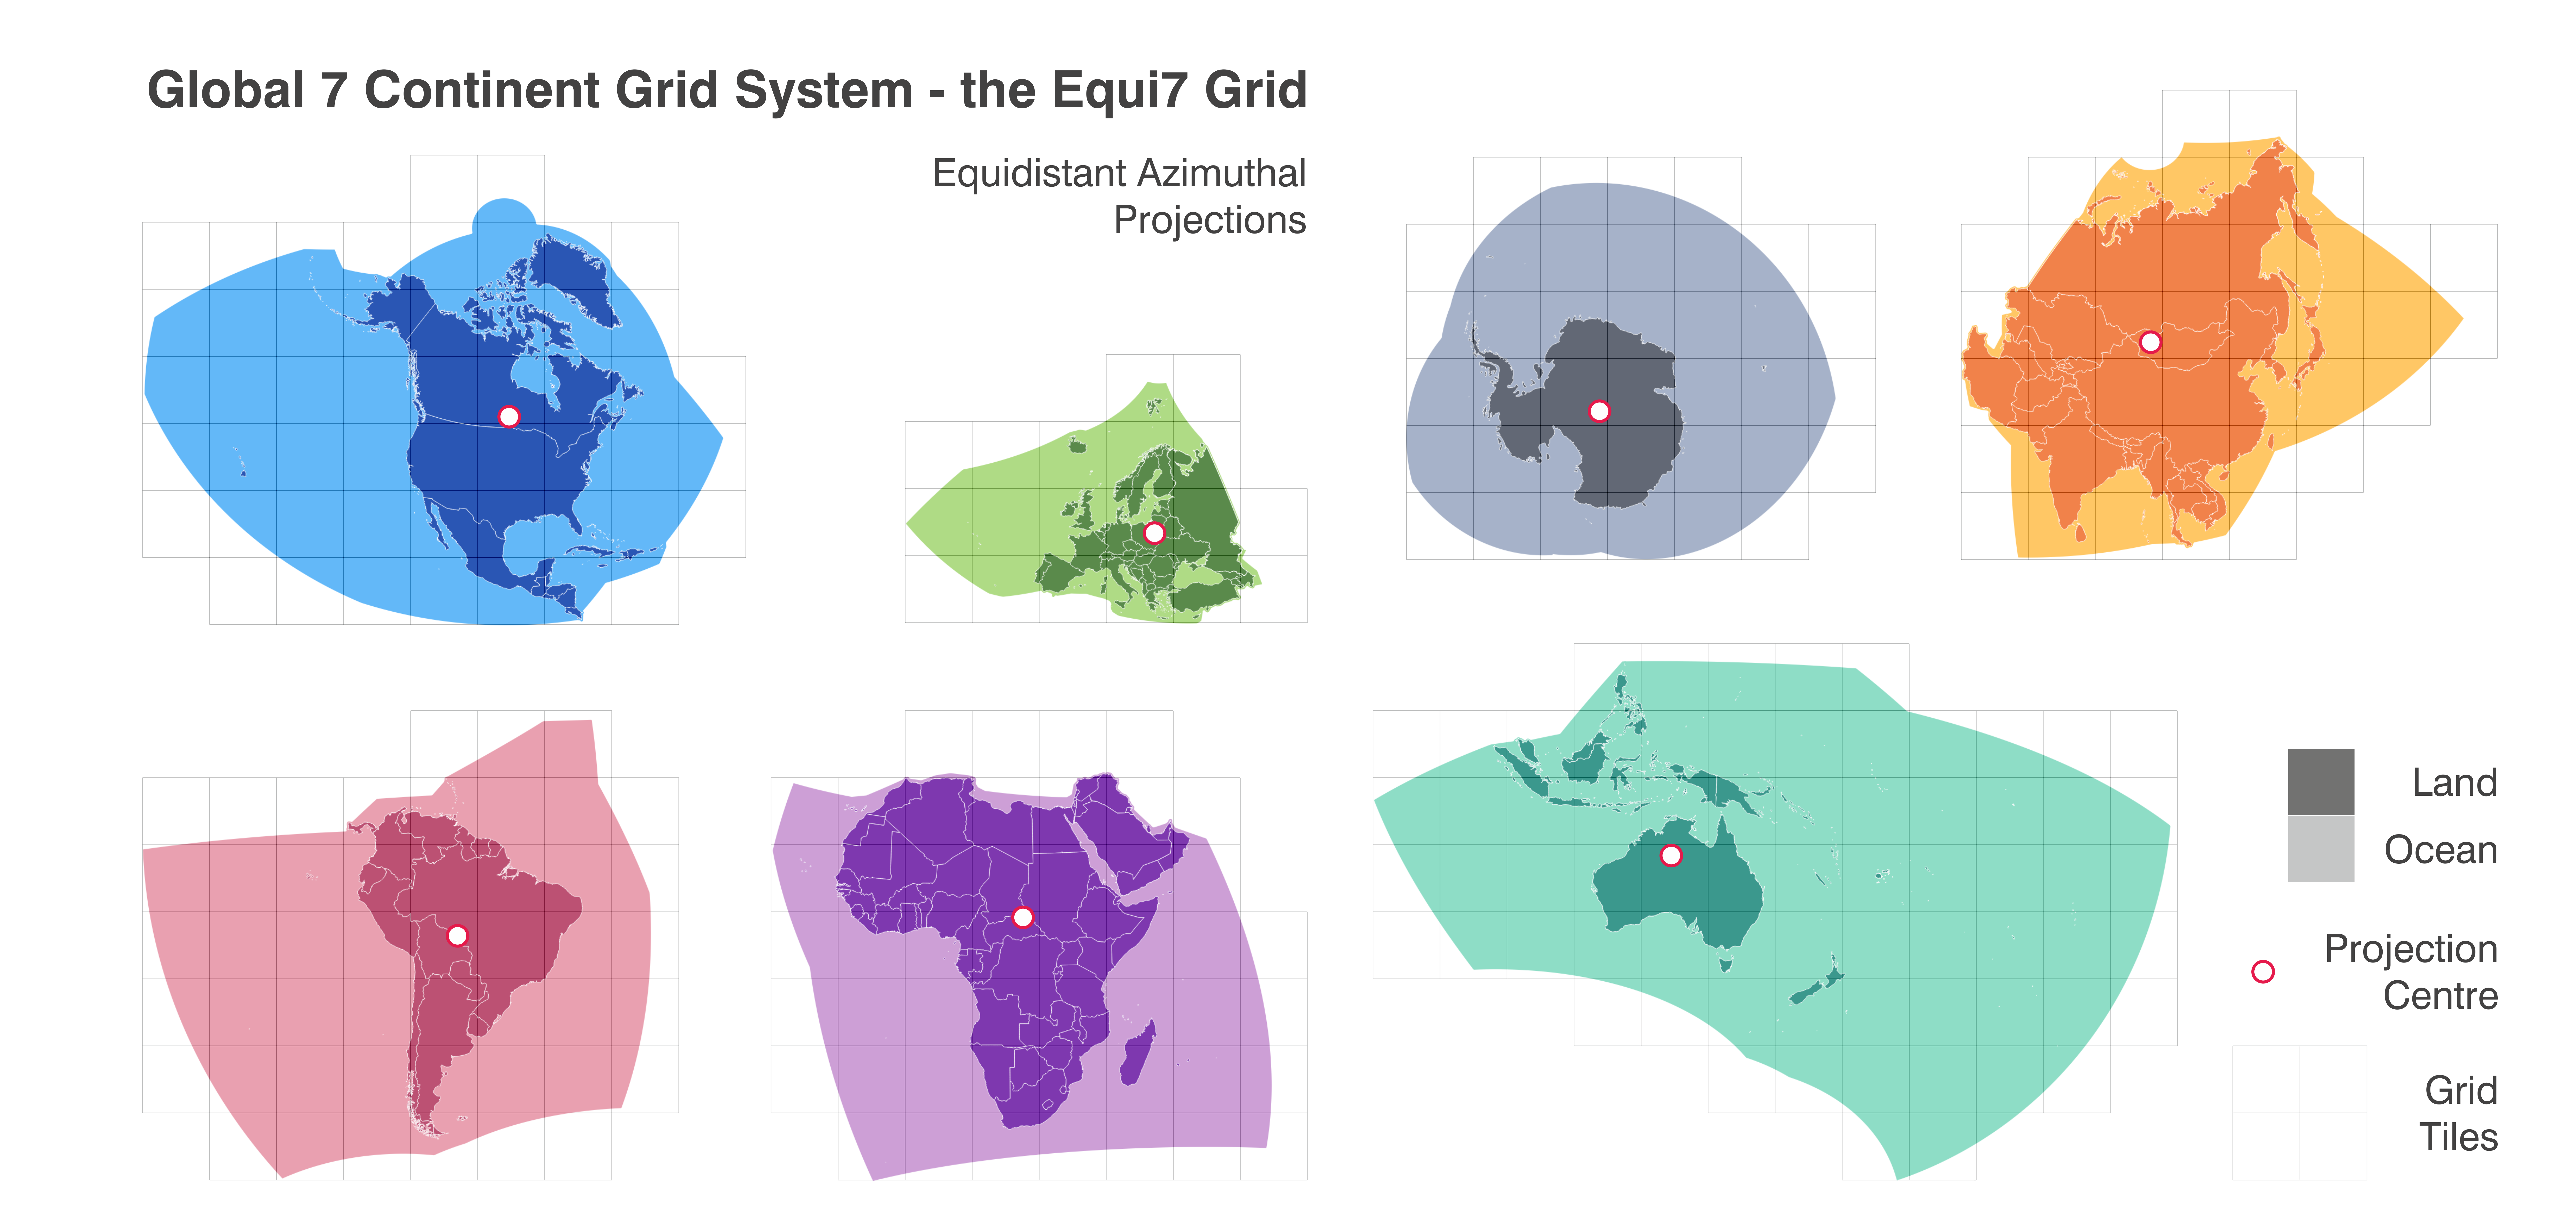
\includegraphics[width=1.0\textwidth]{7continents_grid_v11}
\caption{
The Equi7 Grid: Schematic images of the (already projected) continental zones with grid tiles and projection centres.
}
\label{fig:7cont}
\end{figure}

\section{Design and Geometry}
\label{sec:design}

\subsection{Datum}
As spatial reference the WGS84-ellipsoid (World Geodetic System 1984) was chosen for the ellipsoidal coordinates on the Earth's surface. These are necessary for the addressing of locations in the global perspective, e.g. during the assignment of satellite scenes to the subgrids. Here the ellipsoid's metrics:

\begin{table}[hbtp]
\centering
	{
	\begin{tabular}{ll}
	\hline 
	Major Axis \textbf{a} & $6378137 m$ \\
	Flattening \textbf{f} & $298.257223563^{-1}$ \\
	Prime Meridian & $0.0^{\circ}$ \\
	Unit & $0.0174532925199433^{\circ}$ \\
	\hline 
	\end{tabular} 
	}
\caption[Map Projections]{
The WGS84 Ellipsoid parameters
}
\label{tab:wgs84}
\end{table}

\subsection{Zones}
The Equi7 Grid is a regular grid which defines each location implicitly with a fixed sampling distance relative to a set of linear axis; here two orthogonal ones. As opposed to a single grid for the whole globe, Equi7 separates the globe into seven subgrids (zones) of identical type of projection. Reducing the extent of a projected grid (in respect to the Earth curvature) reduces negative effects from geometric distortions, like data oversampling or disordered pixel neighbour relationships.

Considering findings of the study of \citep{Bauer-Marschallinger2014}, and with TU-Wien's processor- and user requirements in mind, the zone borders were optimised by following requirements: 
\begin{enumerate}
\item Landmasses should form compact entities
\item Borders should be preferably over oceans
\item Countries should preferably be not split
\end{enumerate}

The seven grids cover the Earth entirely without gap and with 50km overlap over land borders. A global overview of the delineation is shown in Figure \ref{fig:gridzones}.

\begin{figure}[hbtp]
\centering
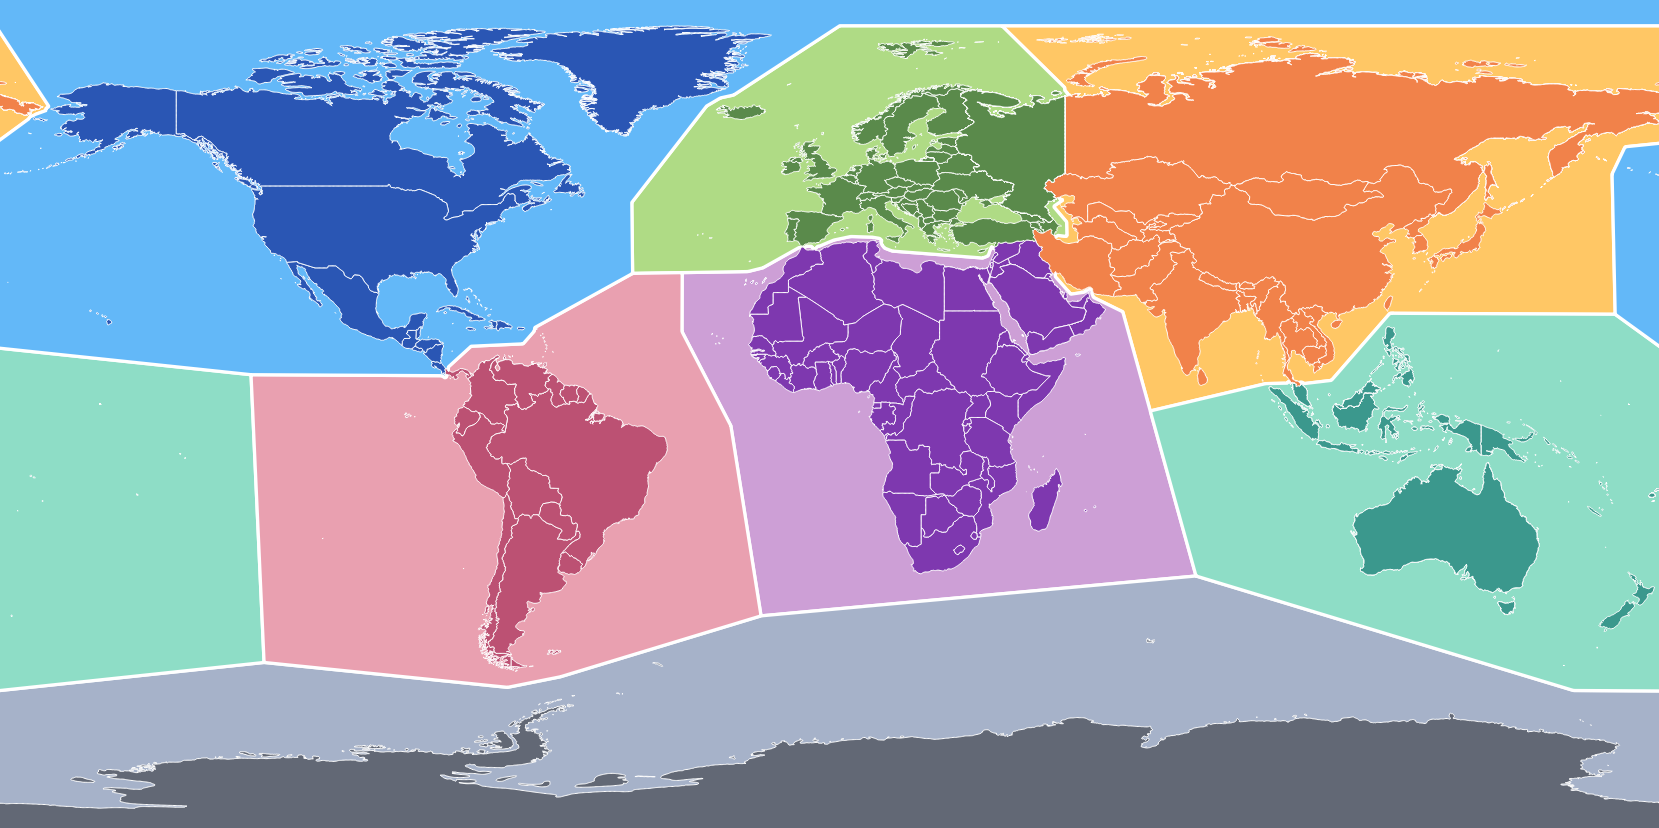
\includegraphics[width=1.0\textwidth]{equi7_grid_v11_overview}
\caption{
Continental zone partitioning into the seven subgrids, projected for global overview to the Plate Carr\'{e}e (aka geographic aka Lat-Lon, using WGS84 coordinates).
}
\label{fig:gridzones}
\end{figure}

The zones are defined by manually created shapefiles following above rules 1-3 in the WGS84 space. After transformation to the individual projections (see Section \ref{sub:projections}), zone borders over land are buffered to a 50km extent to allow correct spatial filter operations also on the zone limits. Table \ref{tab:zones} lists the zones' basic facts. 

\begin{table}[hbtp]
\centering
	{
	\begin{tabular}{lccr}
	\textbf{Zone} & \textbf{Short Name} & \textbf{Colour} & \textbf{Covered Land Area} \\
	& & & [Mio. km$^{2}$] \\
	\hline
	North America & NA & blue & 24.2 \\
	Europe & EU & green & 9.7 \\
	Asia & AS & orange & 38.6 \\
	South America & SA & red & 17.9 \\
	Africa & AF & purple & 33.6 \\
	Oceania & OC & turquoise & 11.2 \\
	Antarctica & AN & gray & 12.3 \\
	\hline
	\end{tabular} 
	}
\caption[Zone Facts]{
The Equi7 Grid zones.
}
\label{tab:zones}
\end{table}

\newpage

\subsection{Projections}
\label{sub:projections}

All seven zone are projected from ellipsoidal coordinates (lat/lon) in WGS84 to planar grids using the \textit{Equidistant Azimuthal Projection}. Figure \ref{fig:equi_azi} exemplifies the projection in oblique aspects. 

\subsubsection{The Azimuthal Equidistant}

\begin{figure}[hbtp]
\centering
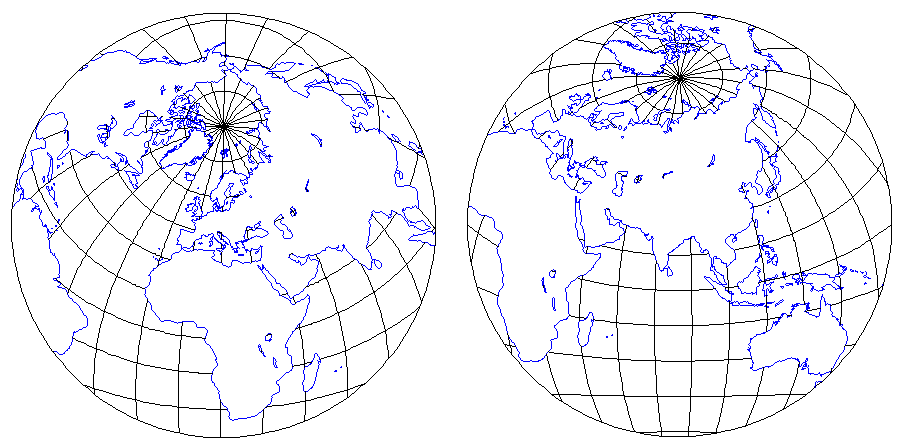
\includegraphics[width=0.9\textwidth]{equi_azi}
\caption{
The Azimuthal Equidistant Projection in oblique aspect centred over Austria (left) and Nepal (right). Linear scales emanating from the projection centre are undistorted. Distortion of angles and areas increases with distance to the centre.
}
\label{fig:equi_azi}
\end{figure}

The calculation of the planar coordinates $x$ and $y$ (the \textit{forward projection}) implies the solving of the \textit{inverse geodesic problem}, that is

\begin{eqnarray}
dx &=& c \sin Az \\ 
dy &=& c \cos Az \\
x &=& dx + FE \\
y &=& dy + FN
\end{eqnarray}

where $x$ and $y$ the are location's Easting and Northing, $c$ is the length and \textit{Az} is the azimuth from north of the geodesic line between the location and the projection centre ($\phi_{0}$, $\lambda_{0}$), $FE$ the false Easting, and $FN$ the false Northing. The \textit{inverse projection} from planar to ellipsoidal coordinates (geodetic latitude $\phi$ and longitude $\lambda$) depicts the \textit{direct geodetic problem} and starts with the determination of \textit{Az} and $c$:

\begin{eqnarray}
dx &=& x - FE \\
dy &=& y - FN \\
\mathit{Az} &=& \arctan \dfrac{dy}{dx} \\
c &=& \sqrt{dx^2 + dy^2}
\end{eqnarray}

Both, the forward and inverse projection of the ellipsoid involve the solving of elliptic integrals that are favourably computed with numerical methods. \cite{Snyder1987} gives approximating formulae and general information on the projection. However, these formulae lead to significant geometric inaccuracies in areas far from the projection centre. Thus, a more recent approach following findings of \citep{Karney2011, Karney2013} is selected for the transformation between geographical and projected coordinates (degrees and metres; see Section \ref{sub:proj_impl}).

\subsubsection{Equi7 Projections}

The parameters of the Azimuthal Equidistant have been individually optimised in means of minimising data oversampling estimated by the mean \textit{grid oversampling factor} as described in \cite{Bauer-Marschallinger2014}. The optimised parameters for each zone are listed in Table \ref{tab:projections}. For Antarctica, the South Pole is conveniently chosen as origin, since it is almost co-located with the the optimal origin and the additional error is insignificant. False Easting and -Northing are set so that negative coordinates are avoided. 

\begin{table}[hbtp]
\centering
	{
	\begin{tabular}{lrrrr}
	\hline
	Parameter & $\mathbf{\lambda_{0}}$ & $\mathbf{\phi_{0}}$ & False Easting & False Northing \\
	Zone / Unit & $^{\circ}E$ & $^{\circ}N$ & m & m \\
	\hline
	North America & $-111.0$ & $47.5$ & $8264722.18$ & $4867518.35$ \\
	Europe & $24.0$ & $53.0$ & $5837287.82$ & $2121415.70$ \\
	Asia & $94.0$ & $47.0$ & $4340913.85$ & $4812712.92$ \\
	South America & $-60.5$ & $-14.0$ & $7257179.24$ & $5592024.45$ \\
	Africa & $21.5$ & $8.5$ & $5621452.02$ & $5990638.42$ \\
	Oceania & $131.5$ & $-19.5$ & $6988408.54$ & $7654884.54$ \\
	Antarctica & $0.0$ & $-90.0$ & $3714266.98$ & $3402016.51$ \\
	\hline
	\end{tabular} 
	}
\caption[Projection Parameter]{
The Equi7 Grid projection parameters for the Azimuthal Equidistant. With $\lambda_{0}$ as central meridian and $\phi_{0}$ as latitude of origin.
}
\label{tab:projections}
\end{table}

The individual \textit{Well-Known-Text}-strings giving the full georeference information are the following:

\subsubsection*{America}

\begin{lstlisting}
PROJCS["Azimuthal_Equidistant",GEOGCS["GCS_WGS_1984",DATUM["D_WGS_1984",SPHEROID["WGS_1984",6378137.0,298.257223563]],PRIMEM["Greenwich",0.0],UNIT["Degree",0.0174532925199433]],PROJECTION["Azimuthal_Equidistant"],PARAMETER["false_easting",8264722.17686],PARAMETER["false_northing",4867518.35323],PARAMETER["central_meridian",-97.5],PARAMETER["latitude_of_origin",52.0],UNIT["Meter",1.0]]
\end{lstlisting}

\subsubsection*{Europe}

\begin{lstlisting}
PROJCS["Azimuthal_Equidistant",GEOGCS["GCS_WGS_1984",DATUM["D_WGS_1984",SPHEROID["WGS_1984",6378137.0,298.257223563]],PRIMEM["Greenwich",0.0],UNIT["Degree",0.0174532925199433]],PROJECTION["Azimuthal_Equidistant"],PARAMETER["false_easting",5837287.81977],PARAMETER["false_northing",2121415.69617],PARAMETER["central_meridian",24.0],PARAMETER["latitude_of_origin",53.0],UNIT["Meter",1.0]]
\end{lstlisting}

\subsubsection*{Asia}

\begin{lstlisting}
PROJCS["Azimuthal_Equidistant",GEOGCS["GCS_WGS_1984",DATUM["D_WGS_1984",SPHEROID["WGS_1984",6378137.0,298.257223563]],PRIMEM["Greenwich",0.0],UNIT["Degree",0.0174532925199433]],PROJECTION["Azimuthal_Equidistant"],PARAMETER["false_easting",4340913.84808],PARAMETER["false_northing",4812712.92347],PARAMETER["central_meridian",94.0],PARAMETER["latitude_of_origin",47.0],UNIT["Meter",1.0]]
\end{lstlisting}

\subsubsection*{South America}

\begin{lstlisting}
PROJCS["Azimuthal_Equidistant",GEOGCS["GCS_WGS_1984",DATUM["D_WGS_1984",SPHEROID["WGS_1984",6378137.0,298.257223563]],PRIMEM["Greenwich",0.0],UNIT["Degree",0.0174532925199433]],PROJECTION["Azimuthal_Equidistant"],PARAMETER["false_easting",7257179.23559],PARAMETER["false_northing",5592024.44605],PARAMETER["central_meridian",-60.5],PARAMETER["latitude_of_origin",-14.0],UNIT["Meter",1.0]]
\end{lstlisting}

\newpage

\subsubsection*{Africa}

\begin{lstlisting}
PROJCS["Azimuthal_Equidistant",GEOGCS["GCS_WGS_1984",DATUM["D_WGS_1984",SPHEROID["WGS_1984",6378137.0,298.257223563]],PRIMEM["Greenwich",0.0],UNIT["Degree",0.0174532925199433]],PROJECTION["Azimuthal_Equidistant"],PARAMETER["false_easting",5621452.01998],PARAMETER["false_northing",5990638.42298],PARAMETER["central_meridian",21.5],PARAMETER["latitude_of_origin",8.5],UNIT["Meter",1.0]]
\end{lstlisting}

\subsubsection*{Oceania}

\begin{lstlisting}
PROJCS["Azimuthal_Equidistant",GEOGCS["GCS_WGS_1984",DATUM["D_WGS_1984",SPHEROID["WGS_1984",6378137.0,298.257223563]],PRIMEM["Greenwich",0.0],UNIT["Degree",0.0174532925199433]],PROJECTION["Azimuthal_Equidistant"],PARAMETER["false_easting",5621452.01998],PARAMETER["false_northing",5990638.42298],PARAMETER["central_meridian",21.5],PARAMETER["latitude_of_origin",8.5],UNIT["Meter",1.0]]
\end{lstlisting}

\subsubsection*{Antarctica}

\begin{lstlisting}
PROJCS["Azimuthal_Equidistant",GEOGCS["GCS_WGS_1984",DATUM["D_WGS_1984",SPHEROID["WGS_1984",6378137.0,298.257223563]],PRIMEM["Greenwich",0.0],UNIT["Degree",0.0174532925199433]],PROJECTION["Azimuthal_Equidistant"],PARAMETER["false_easting",3714266.97719],PARAMETER["false_northing",3402016.50625],PARAMETER["central_meridian",0.0],PARAMETER["latitude_of_origin",-90.0],UNIT["Meter",1.0]]
\end{lstlisting}

\newpage

\section{Production and Structure}
\label{sec:production}

\subsection{Projection Implementation}
\label{sub:proj_impl}

At TU Wien, the Equi7-projections are computed with a python software on a Linux system, using \textit{PROJ.4} via \textit{GDAL/OGR}.

The Equi7 uses a precise algorithm including iterations, as described in \cite{Karney2013}, yielding effectively following equation for inverse and direct geodetic problem, here in the python-notation of the \textit{GeographicLib} library:

\begin{eqnarray}
\left[ c, \mathit{Az} \right] &=& \mathrm{Geodesic.WGS84.Inverse}(\phi_{0}, \lambda_{0}, \phi, \lambda) \\
\left[ \phi , \lambda \right] &=& \mathrm{Geodesic.WGS84.Direct}(\phi_{0}, \lambda_{0}, \mathit{Az}, c)
\end{eqnarray}

Above formulae (including formulae from Section \ref{sub:projections}) are implemented in a modified version of the \textit{proj-4.8.0} library, replacing the approximating formulae of \citep{Snyder1987} in the source code file

\texttt{PJ\_aeqd.c}. 

Those are called via \textit{GDAL/OGR 1.10.0}. The enhancements were reported to the proj.4 project so that it will be included in upcoming releases. In the meantime (Equi7 V12, November 2014), a batch for Linux systems, 

\texttt{proj-4.8.0\_tu\_wien\_batch.zip},

is set up to apply all necessary changes to the official release of proj.4. As a note, the resulting Equi7 shapefiles and DEMs are practically identical to results produced with \textit{ArcGIS 10.2} via its Python module \textit{arcpy}.

\newpage

\subsection{Grid Defining Files}
\label{definingfiles}

The Equi7 Grid Version 12 Public Package constitutes of these shapefiles that come with the projection files:

\paragraph{Zone Shapefile in Equi7 space}
\texttt{EQUI7\_V11\_CO\_PROJ\_ZONE.shp}

\paragraph{Zone Shapefile in Lat/Lon space}
\texttt{EQUI7\_V11\_CO\_PROJ\_ZONE.shp}

A (vector-) shapefile determining the outline of the continental subgrids. \texttt{CO} holds place for the continent name. \texttt{proj} for the coordinate space.

\paragraph{Land Shapefile in Equi7 space}
\texttt{EQUI7\_V11\_CO\_PROJ\_LAND.shp}

\paragraph{Land Shapefile in Lat/Lon space}
\texttt{EQUI7\_V11\_CO\_GEOG\_LAND.shp}

A (vector-) shapefile describing the country borders as provided by the \textit{TM\_WORLD\_ BORDERS-0.3}.

\bibliographystyle{model2-names}
\bibliography{Equi7_Grid_v11_Documentation}

\end{document}
